\documentclass[9pt,twocolumn]{article}

\usepackage[margin=.5in]{geometry}
\usepackage{sectsty}
\usepackage{graphicx}
\usepackage{caption}
\usepackage{listings}

\title{
  \textbf{CMSC 132: Computer Architecture} \\
  First Examination Reviewer
}
\date{}
\sectionfont{\centering\fontsize{12}{14}\selectfont}
\subsectionfont{\fontsize{10}{10}\selectfont}
\captionsetup{justification=centering}
\pagenumbering{gobble}
\lstset{
  basicstyle={\ttfamily},
  breaklines=true,
  showstringspaces=false,
  breakatwhitespace=true
}

\begin{document}
\maketitle

\section*{Computer Architecture in a Nutshell}
  Some concerns:
  \begin{itemize}
    \item How are commands/instructions represented?
    \item What commands/instructions are included?
    \item How much memory is needed?
    \item What is the priority: speed, efficiency or cost?
  \end{itemize}

\section*{Computer History}
  Electronic computers as we know them today began in around 1940s to 1950s.
  \begin{figure}[h]
    \centering
    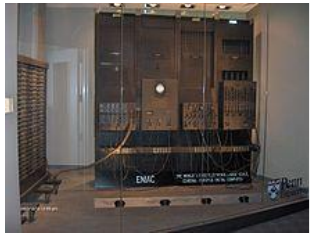
\includegraphics[scale=0.75]{./assets/001/eniac.png}
    \caption{Electronic Numerical Integrator And Computer (ENIAC)}
  \end{figure}

  Computers were done for some specific purpose contrary to a general purpose computer we understand today.
  \begin{itemize}
    \item Decrypting/Encrypting messages
    \item Numeric computing
    \item Business computation
  \end{itemize}
  
\section*{Electric Current Controllers}
  \subsection*{Vacuum Tube}
  \begin{itemize}
    \item Diodes, triodes, etc.
    \item Vacuum tubes are:
      \begin{enumerate}
        \item unreliable
        \item has high electric consumption
        \item gives off too much heat
      \end{enumerate}
  \end{itemize}
  
  \subsection*{Transistor}
  \begin{itemize}
    \item less power consumption
    \item smaller compared with vacuum tubes
    \item greater reliability compared with vacuum tubes
  \end{itemize}
  
  \subsection*{Integrated Circuit}
  \begin{itemize}
    \item smaller and lighter compared with transistors
    \item more reliable compared with transistors
  \end{itemize}
  
  \begin{figure}[h]
    \centering
    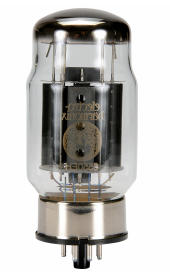
\includegraphics[scale=0.4]{./assets/001/vacuum-tube.png}
    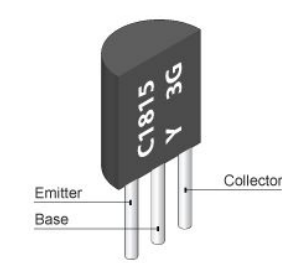
\includegraphics[scale=0.4]{./assets/001/transistor.png}
    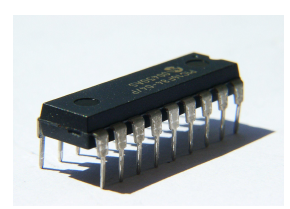
\includegraphics[scale=0.5]{./assets/001/integrated-circuit.png}
    \caption{Images of Vacuum Tube, Transistor, and Integrated Circuit}
  \end{figure}
  
\section*{Computer Architecture}
  According to Wikipedia (Accessed 2013), Computer Architecture "is a \textbf{set of disciplines that describes a computer system by specifying its parts and their relations}."
  \begin{itemize}
    \item Coined by IBM in 1964 for the use with the IBM 360.
    \item Used by \textbf{Amdahl}, \textbf{Blaauw} and \textbf{Brooks} used the term to refer to the programmer-visible portion of the instruction set.
    \item Machines with same architecture must be able to run the same software.
    \item Defined architecture as the \emph{structure of a computer that a machine language programmer must understand to write a correct (timing independent) program for that machine}.
    \item Those who design computers must be proficient in computer architecture.
      \begin{enumerate}
        \item Determine what attributes of a new computer are important
        \item Design the computer to maximize efficiency and performance considering power, availability and cost
        \item Define what instructions are supported, how much memory used, etc. (ISA)
      \end{enumerate}
  \end{itemize}

\section*{Instruction Set Architecture (ISA)}
  \begin{itemize}
    \item The "actual programmer-visible instruction set"
    \item Boundary between the hardware and the software
      \begin{enumerate}
        \item More like an interface between the two
        \item Definition of memory mapping
      \end{enumerate}
    \item Defines what instructions can be understood by the processor
  \end{itemize}

\section*{Seven Dimensions of ISA}
  \subsection*{Class of ISA}
  \begin{itemize}
    \item General-purpose vs special-purpose register architectures
    \item Mostly general-purpose
    \item \textbf{Example:} 80x86 has 16 general-purpose registers and 16 that can hold floating point data
  \end{itemize}

  \subsection*{Memory Addressing}
  \begin{itemize}
    \item Virtually all desktop and server computers, including the 80x86 and MIPS, use byte addressing to access memory operands
    \item Some (e.g., ARM, MIPS) require to be aligned.
    \item An access to an object of size s bytes at byte address A is aligned if A mod s = 0.
    \item Aligned operands are generally faster.
  \end{itemize}

  \subsection*{Addressing Modes}
  \begin{itemize}
    \item Specify the address of a memory object, registers and constant operands
    \item Examples:
      \subitem Immediate (\texttt{add R1, 5})
      \subitem Register (\texttt{add R1, R2})
      \subitem Displacement (\texttt{add R1, 100(R2)})
  \end{itemize}

  \subsection*{Types and Sizes of Operands}
  \begin{itemize}
    \item 8-bit (ASCII character)
    \item 16-bit (Unicode character or half word)
    \item 32-bit (integer or word)
    \item 64-bit (double word or long integer)
    \item IEEE 754 floating point in 32-bit (single precision) and 64-bit (double precision).
  \end{itemize}

  \subsection*{Operands}
  The general categories of operations are data transfer, arithmetic, logical, control, and floating point.

  \subsection*{Control Flow Instructions}
  The support for conditional branches, unconditional jumps, procedure calls, and returns. \textbf{Example:} \texttt{BE}, \texttt{BNE}

  \subsection*{Encoding an ISA}
  \begin{itemize}
    \item There are two basic choices on encoding: fixed length and variable length.
    \item Variable length instructions can take less space compared with fixed-length.
  \end{itemize}

\section*{The Von Neumann Architecture}
  Proposed by \textbf{John von Neumann}, American-Hungarian which is a design architecture for an electronic digital computer; a single memory, stored program architecture based on von Neumann’s paper.
  \begin{figure}[h]
    \centering
    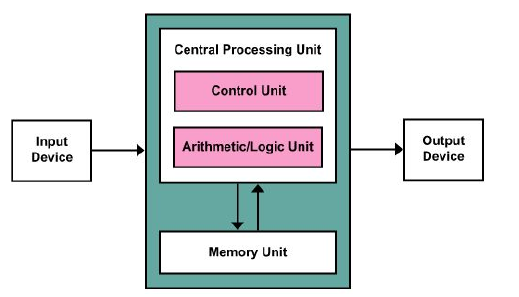
\includegraphics[scale=0.6]{./assets/001/von-neumann.png}
    \caption{The Von Neumann Architecture}
  \end{figure}

  \subsection*{Arithmetic Logic Unit (ALU)}
    It is the digital circuit responsible for different arithmetic and logical operations.
    \begin{figure}[h]
      \centering
      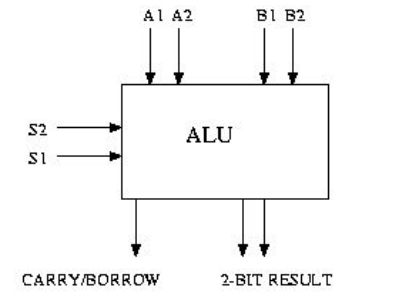
\includegraphics[scale=0.5]{./assets/001/alu.png}
      \caption{Arithmetic Logic Unit (ALU)}
    \end{figure}

  \subsection*{Control Unit (CU)}
    It is responsible for "controlling" other components’ (memory, ALU, etc.) behavior so that instructions are executed properly.
    Things that needed to be remembered:
    \begin{itemize}
      \item Instruction Register (IR)
      \item Program Counter (PC)
      \item Memory Address Register (MAR)
    \end{itemize}

  \subsection*{Memory}
    It is responsible for storing data.

  \subsection*{Input/Output}
    They are devices that serve as an interface to communicate with the user

\section*{Architecture and Organization}
  \subsection*{Architecture}
    \begin{itemize}
      \item Those attributes visible to the programmer
      \item Covers Instruction set, number of bits used for data representation, I/O mechanisms, addressing techniques.
    \end{itemize}

  \subsection*{Organization}
    \begin{itemize}
      \item How features are implemented
      \item Covers control signals, interfaces, memory technology.
    \end{itemize}

  \subsection*{Structure}
    Structure is the way in which components relate to each other.

  \subsection*{Function}
    Function is the operation of individual components as part of the structure.
    All computer functions are:
    \begin{itemize}
      \item Data Processing
      \item Data Storage
      \item Data Movement
      \item Control
    \end{itemize}

    \begin{figure}[h]
      \centering
      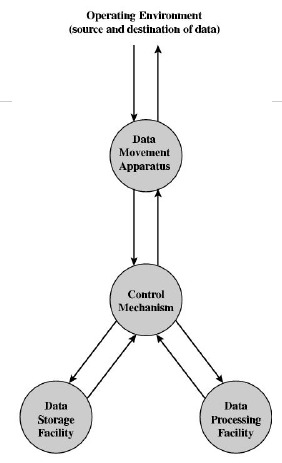
\includegraphics[scale=0.6]{./assets/001/fxn-view.png}
      \caption{Function View}
    \end{figure}

    \begin{figure}[h]
      \centering
      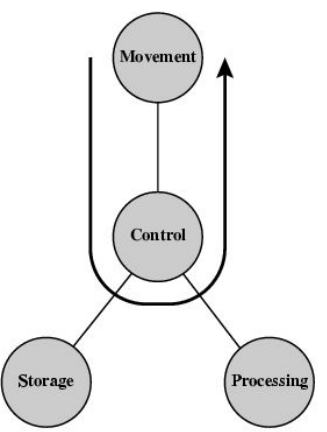
\includegraphics[scale=0.4]{./assets/001/data-movement.png}
      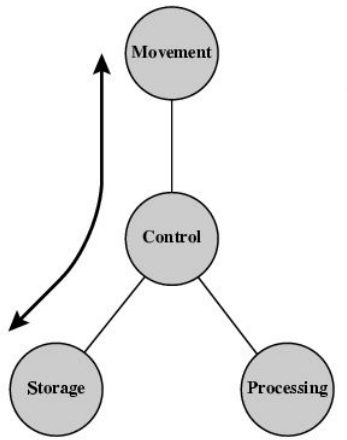
\includegraphics[scale=0.4]{./assets/001/storage.png}
      \caption{Data Movement and Storage}
    \end{figure}

    \begin{figure}[h]
      \centering
      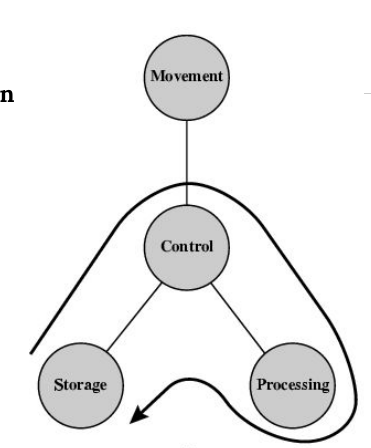
\includegraphics[scale=0.4]{./assets/001/processing-to-storage.png}
      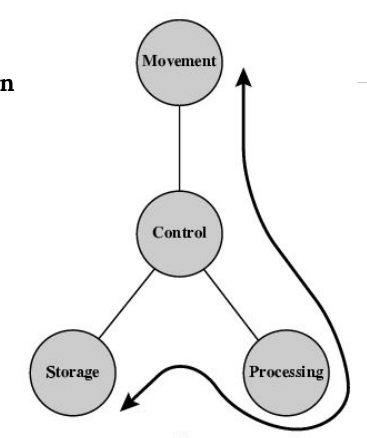
\includegraphics[scale=0.4]{./assets/001/processing-from-io.png}
      \caption{Processing to/from Storage and Processing from Storage to I/O}
    \end{figure}

    \begin{figure}[h!]
      \centering
      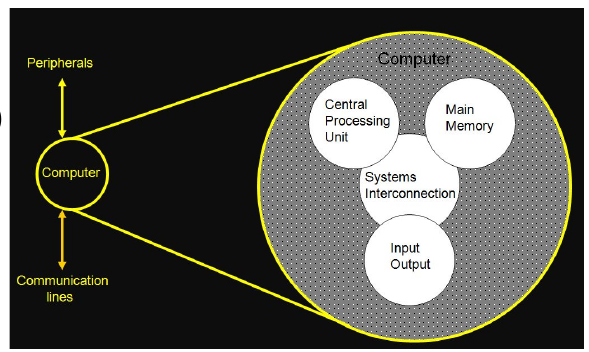
\includegraphics[scale=0.5]{./assets/001/struct-top.png}
      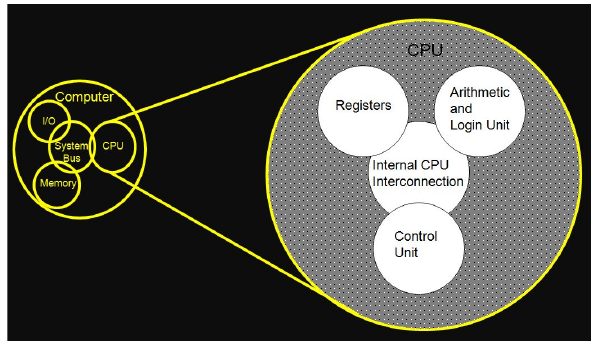
\includegraphics[scale=0.5]{./assets/001/struct-cpu.png}
      \caption{Structure: Top Level and CPU}
    \end{figure}

\section*{The Fetch-Decode-Execute (FDE) Cycle}
  It is the process of getting program instruction, decoding the instruction through appropriate paths and executing the instruction.

  \subsection*{Fetch}
    \begin{enumerate}
      \item The address of the first instruction is pointed to by \textbf{PC}.
      \item The \textbf{MAR} holds the address pointed to by \textbf{PC}.
      \item \textbf{PC} (or the address held inside it) is incremented by one.
      \item The instruction is fetched from memory; the data is copied to the \textbf{MDR}.
    \end{enumerate}

  \subsection*{Decode}
    \begin{enumerate}
      \item The instruction is determined and prepares appropriate registers for the instruction.
      \item \textbf{Example:} Are there two operands or only one operand? What register(s) was/were used?
    \end{enumerate}

  \subsection*{Execute}
    \begin{enumerate}
      \item The instruction is coursed through the appropriate circuits.
      \item The instruction is executed using the appropriate registers as input (if there are needed operands).
    \end{enumerate}

\section*{Instruction Sets}
  \subsection*{Reduced Instruction Set Computer (RISC)}
    It is a type of microprocessor architecture that utilizes a small, highly-optimized set of instructions, rather than a more specialized set of instructions often found in other types of architectures.

  \subsection*{Complex Instruction Set Computer (CISC)}
    CISC are chips that are easy to program and which make efficient use of memory.

  \begin{table}[h]
    \centering
    \begin{tabular}{p{4cm} | p{4cm}}
      \textbf{CISC} & \textbf{RISC} \\
      \hline
      Emphasis on hardware & Emphasis on software \\
      Includes multi-clock complex instructions & Single-clock, reduced instruction only \\
      Memory to memory: \texttt{LOAD} and \texttt{STORE} incorporated in instructions & Register to register: \texttt{LOAD} and \texttt{STORE} are independent instructions \\
      Small code sizes, high cycles per second & Low cycles per second, large code sizes \\
      Transistors used for storing complex instrutions & Spends more transistors on memory triggers
    \end{tabular}
  \end{table}

\section*{Machine Models}
  \subsection*{Stack-Based}
    \begin{itemize}
      \item Number of Explicit Operands: 0
      \item Examples
        \subitem HP 3000
        \subitem ICL 2900
        \subitem Java Virtual Machine (modern)
        \subitem Intel x87 Floating Point Unit (modern)
    \end{itemize}
  \subsection*{Accumulator-Based}
    \begin{itemize}
      \item Number of Explicit Operands: 1
      \item Common before 1980s
    \end{itemize}
  \subsection*{Register-Memory}
    \begin{itemize}
      \item Number of Explicit Operands: 2 or 3
      \item Examples
        \subitem VAX
        \subitem 80x86
    \end{itemize}
  \subsection*{Register-Register}
    \begin{itemize}
      \item Number of Explicit Operands: 2 or 3
      \item Examples
        \subitem MIPS
        \subitem SPARC
    \end{itemize}

  \begin{figure}[h]
    \centering
    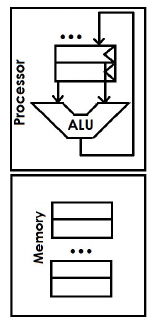
\includegraphics[scale=0.5]{./assets/001/stack.png}
    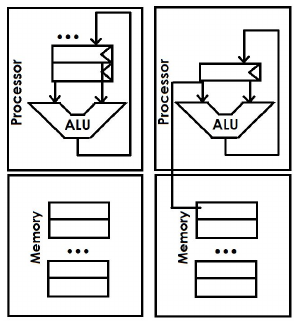
\includegraphics[scale=0.5]{./assets/001/accumulator.png}
    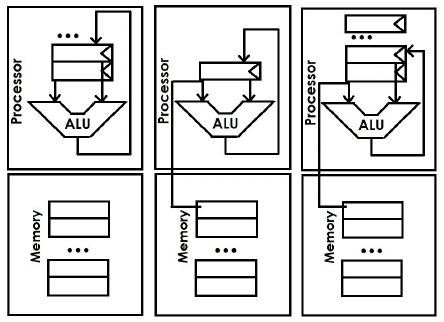
\includegraphics[scale=0.3]{./assets/001/register-memory.png}
    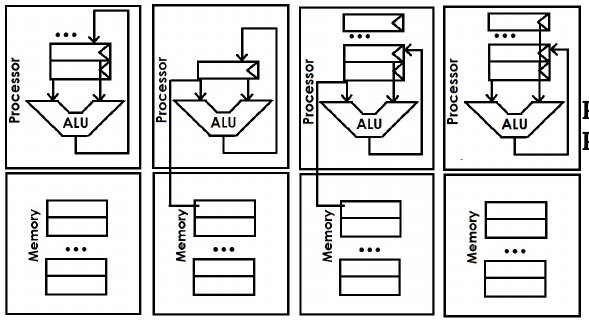
\includegraphics[scale=0.3]{./assets/001/register-register.png}
    \caption{Stack-based, Accumulator-based, Register-Memory, and Register-Register ISA}
  \end{figure}

  \begin{table}[h]
    \centering
    \begin{tabular}{|l|l|}
      \hline
        \multicolumn{1}{|c|}{\textbf{Stack}} & \multicolumn{1}{c|}{\textbf{Accumulator}} \\
      \hline
        \begin{lstlisting}[gobble=10]
          push A
          push B
          add
          pop C
        \end{lstlisting} &
        \begin{lstlisting}[gobble=10]
          load A
          add B
          store C
        \end{lstlisting} \\
      \hline
        \multicolumn{1}{|c|}{\textbf{Register-Memory}} & \multicolumn{1}{c|}{\textbf{Register-Register}} \\
      \hline
        \begin{lstlisting}[gobble=10]
          load R1, A
          add R3, R1, B
          store R3, C
        \end{lstlisting} &
        \begin{lstlisting}[gobble=10]
          load R1, A
          load R2, B
          add R3, R1, R2
          store R3, C
        \end{lstlisting} \\
      \hline
    \end{tabular}
    \caption{Instruction Representation of \texttt{C = A + B} in Different Machine Models}
  \end{table}

\end{document}